\documentclass[../report.tex]{subfiles}

\begin{document}

\usepgfplotslibrary{statistics}

\chapter{Results} % Performance comparison for the KHAPE library (not the password manager use case).

This chapter presents the performances obtained by the implemented KHAPE library using different parameters and analyzing the performance of some of the component. A performance comparison with OPAQUE rust implementation \cite{opaque-ke} is made. The password manager use case is not in the scope of test.

\section{Testing environment}

For computation benchmark, the rust library Criterion is used. It compute each benchmark 100 times.
Each benchmark is sampled 100 times and each sample linearly increase the number of iteration on the tested function.
The median is used for the charts.

The benchmark are computed on a HP Elitebook 850 G5 laptop with an intel i7-8550U processor.\footnote{The laptop is plugged to the charging cable during all the benchmarks. This make a performance gain of around 40\% compared to when it runs on battery.} 





\section{KHAPE components benchmark}

Before diving into the overall performances of KHAPE and its endpoints, it is important to understand what are some of the components that take the most time to compute.

\subsection{3DH}

The 3DH AKE is unsurprisingly the most time consuming operation to compute. Considering that a curve multiplication take around 58 us to compute and that 3DH --- as its name suggest --- compute 3 of them. Adding the cost of derivating 2 keys using HKDF, the median time of 3DH computation is around 184 us.

% TODO HMQV

Both client and server functions has around the same performances. This is not surprising because they compute the same operations with different party's key.

\pgfplotsset{width=\textwidth +0.2cm}
\pgfplotsset{height=6cm}

\begin{tikzpicture}
\begin{axis}[
    boxplot,
    boxplot/draw direction=x,
%     xmin=0.211, xmax=0.232,
    xlabel={microsecond},
    ytick={1,2},
    yticklabels={server,client},
    title=Time consumption of 3DH computation,
]
\addplot table[y=value]{\subfix{data/component/tripledh_compute_server.dat}};
\addplot table[y=value]{\subfix{data/component/tripledh_compute_client.dat}};
\end{axis}
\end{tikzpicture}

Time consumption of a single curve multiplication operation.

\pgfplotsset{width=\textwidth-2.4cm}
\pgfplotsset{height=4cm}

\begin{tikzpicture}
\begin{axis}[
    boxplot,
    boxplot/draw direction=x,
    xmin=57.5, xmax=64.5,
    xlabel={microsecond},
    ytick={1},
    yticklabels={curve multiplication},
    title=Time consumption of one exponentiation,
]
\addplot table[y=value]{\subfix{data/component/group_compute_shared_key.dat}};
\end{axis}
\end{tikzpicture}

\subsection{Key generation}

Key generation take also a lot of time with a median of 122 us. Key generation consist of: 1) generating a 32 bytes random value, 2) generating a private key from the random bytes, 3) computing its associated public key --- a curve multiplication operation --- and then 4) converting the public key to a field element using the elligator2 map.

For step 2, not all 32 bytes random value can be used to generate a private key and for step 4, not all public key can be mapped to a field element.
In these case, the rejection method is used which means that the key generation process is restarted from step 1. This is more secure than trying to modify the value to make it fit but in the other hand, it is more costly in term of performance as the key generation process can be made multiple time.
This is also why the time distribution of this function is more spread out than for other function.

% TODO nombre de fois en moyenne

\pgfplotsset{width=\textwidth-0.3cm}
\pgfplotsset{height=4cm}

\begin{tikzpicture}
\begin{axis}[
    boxplot,
    boxplot/draw direction=x,
%     xmin=0.211, xmax=0.232,
    xlabel={microsecond},
    ytick={1},
    yticklabels={generate},
    title=Time consumption of a key pair generation,
]
\addplot table[y=value]{\subfix{data/component/group_generate_keys.dat}};
\end{axis}
\end{tikzpicture}




\subsection{Encryption scheme}
KHAPE require a Ideal Cipher encryption which has been implemented with a 14-rounds feistel cipher.

\pgfplotsset{width=\textwidth-0.1cm}
\pgfplotsset{height=6cm}

\subsection*{Feistel cipher}

The feistel cipher implemented is not optimal in term of performance but it is surprising not that much time consuming.
It is still around 36 times slower than AES256-CTR (see below) but it doesn't take much time compared to the group operation above.

% TODO encryption and decryption ?
% TODO AES256-CTR performances (HW, para, optimized)

\begin{tikzpicture}
\begin{axis}[
    boxplot,
    boxplot/draw direction=x,
    xmin=7.4, xmax=8.55,
    xlabel={microsecond},
    ytick={1,2},
    yticklabels={decrypt,encrypt},
    title=Time consumption of Feistel cipher operations
]
\addplot table[y=value]{\subfix{data/component/ideal_cipher_decryption.dat}};
\addplot table[y=value]{\subfix{data/component/ideal_cipher_encryption.dat}};
\end{axis}
\end{tikzpicture}

\subsection*{AES256-CTR}
Even though AES cannot be used for the encryption in KHAPE, it is still interesting to benchmark it with the same context that the feistel cipher is used for.

Encryption and decryption take almost exactly the same time in median because with AES-CTR, the decryption is performed with the same function as the encryption.

\begin{tikzpicture}
\begin{axis}[
    boxplot,
    boxplot/draw direction=x,
    xmin=0.211, xmax=0.232,
    xlabel={microsecond},
    ytick={1,2},
    yticklabels={decrypt,encrypt},
    title=Time consumption of AES256-CTR operations
]
\addplot table[y=value]{\subfix{data/component/aes_decryption.dat}};
\addplot table[y=value]{\subfix{data/component/aes_encryption.dat}};
\end{axis}
\end{tikzpicture}





\section{KHAPE benchmark} % What endpoint take the most time during auth and register ? 

In KHAPE, both registration and authentication process have multiple endpoints --- respectively 4 and 5. These endpoints are shared between the client and the server to constitue the protocol.

For this benchmark, each endpoints are tested to mesure the time they take to complete and compare them using different parameters. 
It is interesting to see Section \ref{sec:impl_function_def} to understand what operations are computed on each endpoints and to compare it with the benchmark result.

Note that only the time taken for each endpoints to complete is mesured. In a real world scenario, the resulting messages have to be transmitted between the client and the server. The network delay is not very interesting to benchmark as it depends too much on the network infrastructure between the client and the server. Instead, Section \ref{sec:comp_message_size} shows a comparison of message size between multiple configuration of KHAPE and OPAQUE.

\subsection{Standard configuration}
KHAPE's default and most secure configuration is by using both OPRF and SlowHash. 
But since SlowHash functions are designed to be slow, it doesn't make sense to add it to the baseline benchmark because it doesn't show the real performances of the protocol.
So for these benchmarks, the standard baseline configuration is KHAPE with OPRF and without SlowHash.

\pgfplotsset{width=\textwidth-1.1cm}
\subsection*{Registration}

For the registration, we can see that both \verb|server start| and \verb|client finish| endpoints take the most time at around 200 us.
It is not surprising as it is where each party generate his own key pair, which take around 122 us.

The \verb|server finish| endpoint take almost no time since it only build a storable structure with the value received.

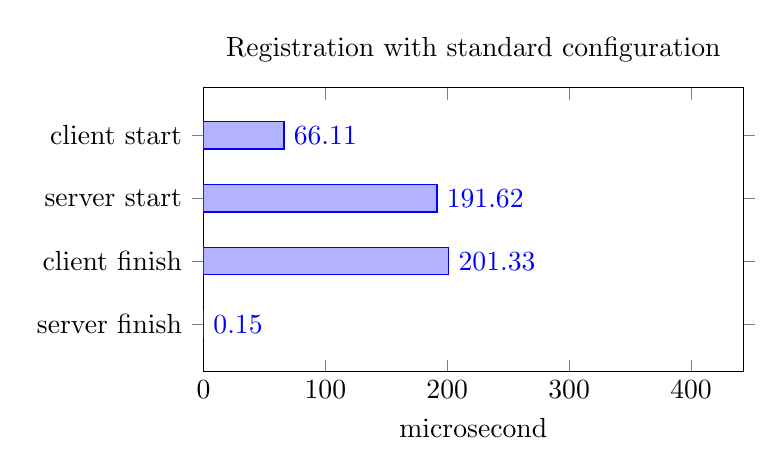
\begin{tikzpicture}
\begin{axis}[
    xbar,
    y=0.8cm,
    xmin=0, xmax=385,
    enlarge y limits=0.25,
    enlarge x limits={0.15, upper},
    legend style={at={(0.5,-0.2)},
    anchor=north,legend columns=-1},
    xlabel={microsecond},
    symbolic y coords={server finish, client finish, server start, client start},
    ytick=data,
    nodes near coords,
    nodes near coords align={horizontal},
    title=Registration with standard configuration,
]
\addplot coordinates {
    (0.15336,server finish)
    (201.33,client finish)
    (191.62,server start)
    (66.105,client start)
};
\end{axis}
\end{tikzpicture}


\subsection*{Authentication}

It is important to note that the endpoints for the registration and authentication are obviously different. For readability reason, it is not specified on the label of the charts but in the chart's title, which could make it looks like authentication and registration share the same function.

We can see that \verb|client ke| endpoint take the most time. This is because a lot of things are computed in this endpoint including the generation of an ephemeral key pair (122 us) and the computation of the 3DH (184 us).

We also notice that both \verb|client start| and \verb|server start| take about the same time than their homonym endpoints in registration. This is because these two functions are relatively similar between registration and authentication.

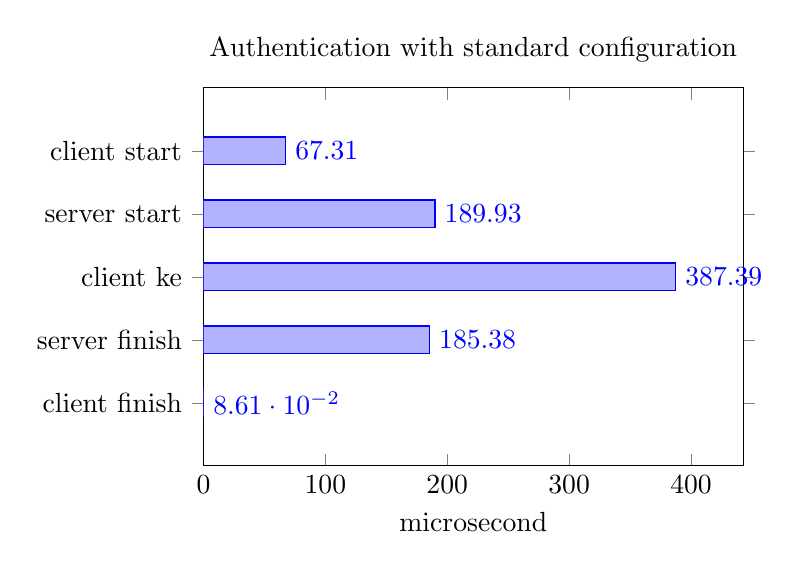
\begin{tikzpicture}
\begin{axis}[
    xbar,
    y=0.8cm,
    xmin=0, xmax=385,
    enlarge y limits=0.25,
    enlarge x limits={0.15, upper},
    legend style={at={(0.5,-0.2)},
    anchor=north,legend columns=-1},
    xlabel={microsecond},
    symbolic y coords={client finish, server finish, client ke, server start, client start},
    ytick=data,
    nodes near coords,
    nodes near coords align={horizontal},
    title=Authentication with standard configuration,
]
\addplot coordinates {
    (0.086069,client finish)
    (185.38,server finish)
    (387.39,client ke)
    (189.93,server start)
    (67.308,client start)
};
\end{axis}
\end{tikzpicture}



% \subsection{Ideal Cipher vs AES} % isolated, endpoints, overall. How does it change the performance of each endpoint and overall ?
% 2 boite à moustache (en mode histogram), x = each endpoint, y = time. Comparison with the standard time (above)

\subsection{With OPRF vs without OPRF} % endpoints, overall. How does it change the performance of each endpoint and overall ?
% 2 boite à moustache (en mode histogram), x = each endpoint, y = time. Comparison with the standard time (above)

OPRF largely increase KHAPE security guarantees (see Section \ref{sec:design_choice_oprf}) but it remains optional.

If used, OPRF is computed for both registration and authentication.
It requires to compute two hashes and three exponentiations (curve multiplication) for each run. The exponentiation are computed on the three first endpoints of registration and authentication.

In this section, we compare the performance of KHAPE with and without OPRF to see how much it impact the overall performances of the protocol.


\subsection*{Registration}

Each OPRF concerned endpoints takes between 66 and 72 us more to compute when using OPRF. In total, the registration will take around 207 us more than without an OPRF.

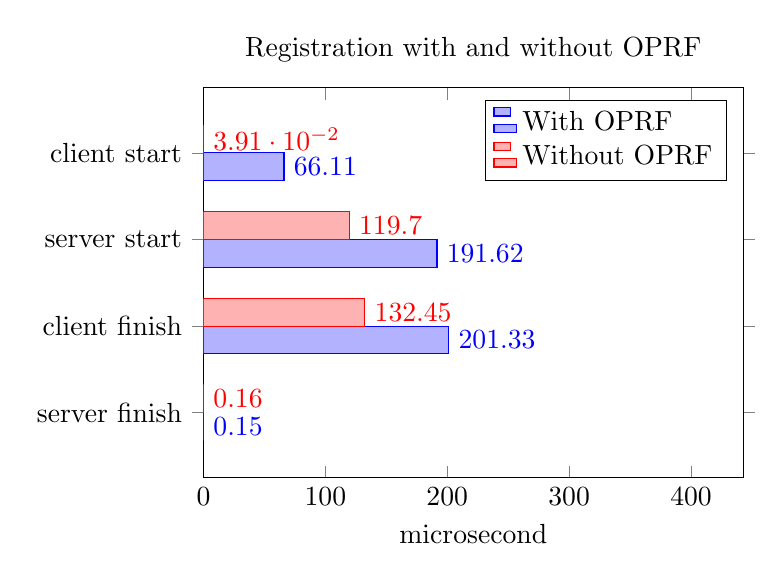
\begin{tikzpicture}
\begin{axis}[
    xbar=0pt,
    y=1.1cm,
    xmin=0, xmax=385,
    enlarge y limits=0.25,
    enlarge x limits={0.15, upper},
    legend pos=north east,
    legend cell align=left,
    xlabel={microsecond},
    symbolic y coords={server finish, client finish, server start, client start},
    ytick=data,
    nodes near coords,
    nodes near coords align={horizontal},
    title=Registration with and without OPRF,
]
\addplot coordinates {
    (0.15336,server finish)
    (201.33,client finish)
    (191.62,server start)
    (66.105,client start)
};
\addplot coordinates {
    (0.15736,server finish)
    (132.45,client finish)
    (119.70,server start)
    (0.039084,client start)
};
\legend{With OPRF,Without OPRF}
\end{axis}
\end{tikzpicture}



\subsection*{Authentication}
For the authentication, it is similar. The first three endpoints take between 67 and 69 us more to compute and the total time addition for the authentication is around 205 us more than without OPRF.

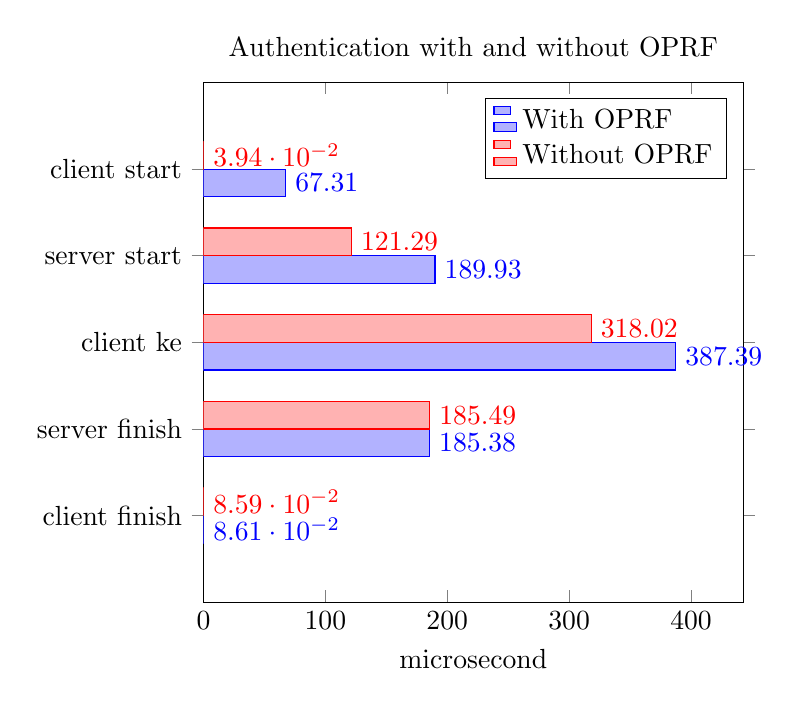
\begin{tikzpicture}
\begin{axis}[
    xbar=0pt,
    y=1.1cm,
    xmin=0, xmax=385,
    enlarge y limits=0.25,
    enlarge x limits={0.15, upper},
    legend pos=north east,
    legend cell align=left,
    xlabel={microsecond},
    symbolic y coords={client finish, server finish, client ke, server start, client start},
    ytick=data,
    nodes near coords,
    nodes near coords align={horizontal},
    title=Authentication with and without OPRF,
]
\addplot coordinates {
    (0.086069,client finish)
    (185.38,server finish)
    (387.39,client ke)
    (189.93,server start)
    (67.308,client start)
};
\addplot coordinates {
    (0.085906,client finish)
    (185.49,server finish)
    (318.02,client ke)
    (121.29,server start)
    (0.039352,client start)
};
\legend{With OPRF,Without OPRF}
\end{axis}
\end{tikzpicture}

\subsection{With SlowHash vs without SlowHash} % endpoints, overall. How does it change the performance of each endpoint and overall ?
% 2 boite à moustache (en mode histogram), x = each endpoint, y = time. Comparison with the standard time (above)

Using a memory-hard hashing function also increase the level of security of the protocol \ref{sec:design_choice_slowhash}.


This benchmark is not very meaningful since these functions are designed to be slow and the performance only depends on the parameters used. But it is still interesting to see the performance degradation attached to the use of these functions and the scale of it compared to the rest of the protocol.

It also make it easier to understand how these functions slow down attackers that build hashing table. Since we replace a simple and efficient hashing function that would not even take 0.5 us to compute by a slow and expansive hashing function that take around 8,000 us to compute. That make it 16,000 time slower to compute and so the attackers can compute 16,000 time less hashes in the same time frame.

This benchmark is using the rust library Argon2's default parameters. The defaults parameters of the KHAPE library are more resource intensive and time consuming since we believe that final user can wait a little bit more than 8 ms to register/authenticate to a secure system.


\subsection*{Registration}

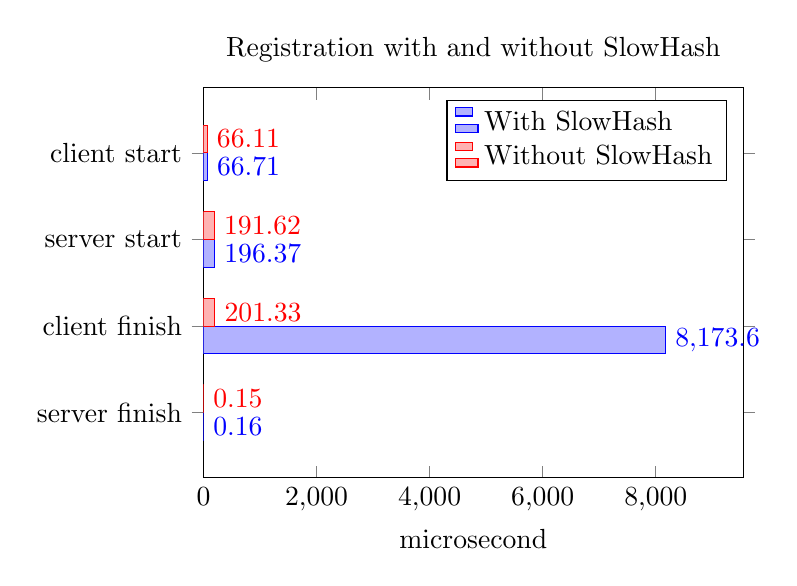
\begin{tikzpicture}
\begin{axis}[
    xbar=0pt,
    y=1.1cm,
    xmin=0, xmax=8300,
    enlarge y limits=0.25,
    enlarge x limits={0.15, upper},
    legend pos=north east,
    legend cell align=left,
    xlabel={microsecond},
    symbolic y coords={server finish, client finish, server start, client start},
    ytick=data,
    nodes near coords,
    nodes near coords align={horizontal},
    title=Registration with and without SlowHash,
]
\addplot coordinates {
    (0.16100,server finish)
    (8173.6,client finish)
    (196.37,server start)
    (66.713,client start)
};
\addplot coordinates {
    (0.15336,server finish)
    (201.33,client finish)
    (191.62,server start)
    (66.105,client start)
};
\legend{With SlowHash,Without SlowHash}
\end{axis}
\end{tikzpicture}



\subsection*{Authentication}

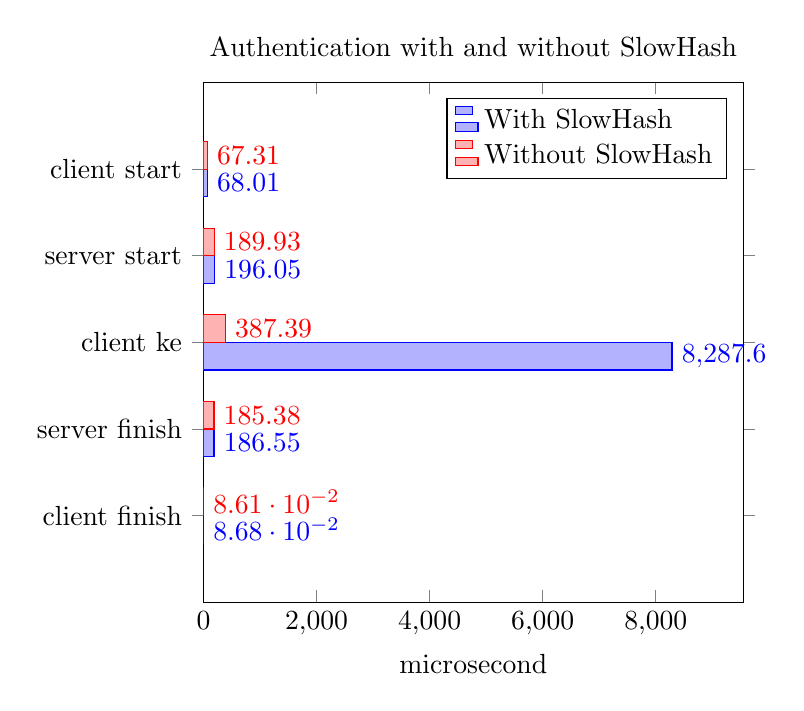
\begin{tikzpicture}
\begin{axis}[
    xbar=0pt,
    y=1.1cm,
    xmin=0, xmax=8300,
    enlarge y limits=0.25,
    enlarge x limits={0.15, upper},
    legend pos=north east,
    legend cell align=left,
    xlabel={microsecond},
    symbolic y coords={client finish, server finish, client ke, server start, client start},
    ytick=data,
    nodes near coords,
    nodes near coords align={horizontal},
    title=Authentication with and without SlowHash,
]
\addplot coordinates {
    (0.086840,client finish)
    (186.55,server finish)
    (8287.6,client ke)
    (196.05,server start)
    (68.013,client start)
};
\addplot coordinates {
    (0.086069,client finish)
    (185.38,server finish)
    (387.39,client ke)
    (189.93,server start)
    (67.308,client start)
};
\legend{With SlowHash,Without SlowHash}
\end{axis}
\end{tikzpicture}





\section{OPAQUE benchmark} % same as KHAPE endpoints. Shows default parameters and similar parameters as KHAPE


KHAPE and OPAQUE designs share lots of similarities. This make OPAQUE a perfect candidate for performances comparison. But before that, we need to understand the difference to be able to compare them fairly.


Benchmark is computed with a ciphersuite that is close to the primitive used for KHAPE : ristretto255 curve for the OPRF group, montgomery cruve for the KE group, 3DH for the AKE and SHA3 for hashing.
Note that the default ciphersuite for OPAQUE use SHA2 instead of SHA3 and ristretto255 curve for both OPRF group and KE group but the performance obtained between the two ciphersuites are relatively similar.

\pgfplotsset{width=\textwidth-1.1cm}


\subsection*{Registration}

For the registration, OPAQUE has an additional endpoint \verb|server setup| that generate the server's key pair. In KHAPE, this operation is done in the \verb|server start| endpoint.

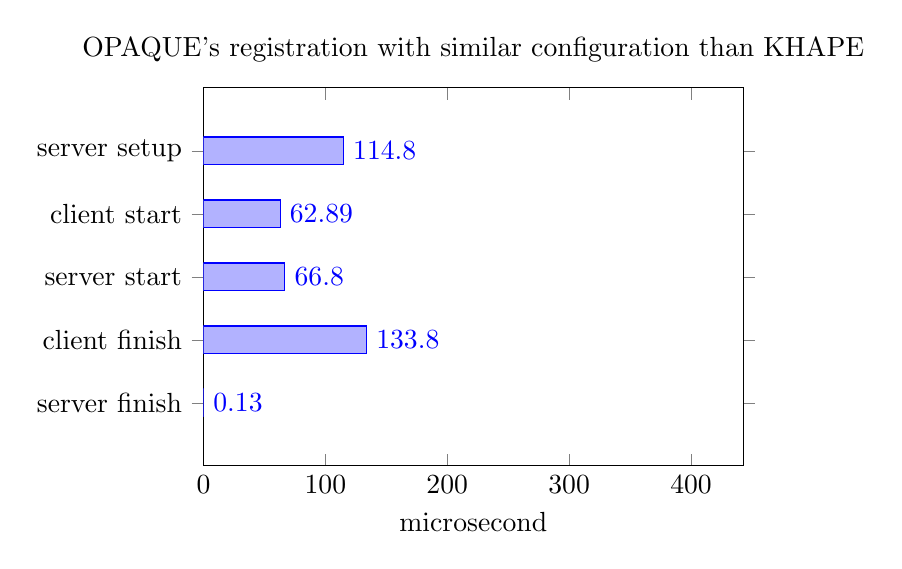
\begin{tikzpicture}
\begin{axis}[
    xbar,
    y=0.8cm,
    xmin=0, xmax=385,
    enlarge y limits=0.25,
    enlarge x limits={0.15, upper},
    legend style={at={(0.5,-0.2)},
    anchor=north,legend columns=-1},
    xlabel={microsecond},
    symbolic y coords={server finish, client finish, server start, client start, server setup},
    ytick=data,
    nodes near coords,
    nodes near coords align={horizontal},
    title=OPAQUE's registration with similar configuration than KHAPE,
]
\addplot coordinates {
    (0.13187,server finish)
    (133.80,client finish)
    (66.797,server start)
    (62.885,client start)
    (114.80,server setup)
};
\end{axis}
\end{tikzpicture}


\subsection*{Authentication}

For the authentication, OPAQUE has only four endpoints since the server initialize the key verification. The \verb|server start| endpoint is the most time consuming with a median time of around 369 us. It is responsible of generating an ephemeral key pair, compute the OPRF evaluation, computing the key exchange and derivating the output key and key verification tag. In KHAPE, all these operations are spread between \verb|server start| and \verb|server finish| endpoints.

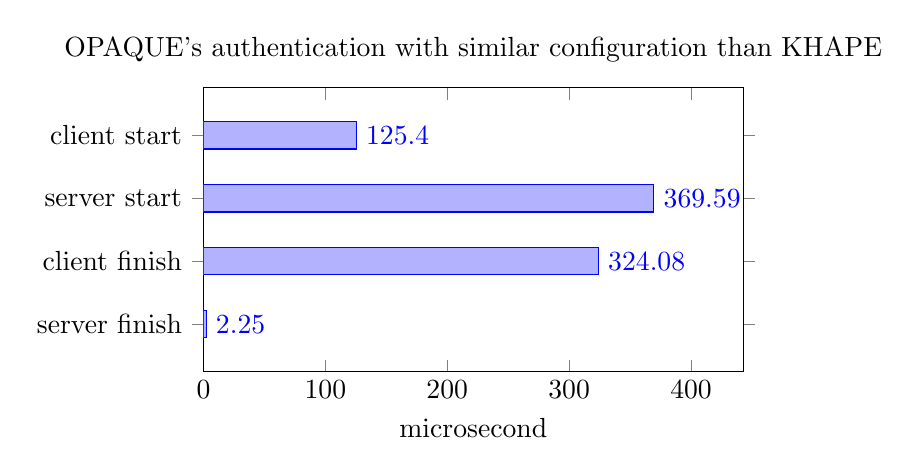
\begin{tikzpicture}
\begin{axis}[
    xbar,
    y=0.8cm,
    xmin=0, xmax=385,
    enlarge y limits=0.25,
    enlarge x limits={0.15, upper},
    legend style={at={(0.5,-0.2)},
    anchor=north,legend columns=-1},
    xlabel={microsecond},
    symbolic y coords={server finish, client finish, server start, client start},
    ytick=data,
    nodes near coords,
    nodes near coords align={horizontal},
    title=OPAQUE's authentication with similar configuration than KHAPE,
]
\addplot coordinates {
    (2.2455,server finish)
    (324.08,client finish)
    (369.59,server start)
    (125.40,client start)
};
\end{axis}
\end{tikzpicture}


\section{OPAQUE vs KHAPE} % endpoints, overall. How does KHAPE performance compare to OPAQUE with ~same~ parameters (OPRF, no SlowHash, same curve ?, same hash ?)
% 2 histogram, one for auth overall, one for register overall, x = OPAQUE(default) OPAQUE(same params) KHAPE(IC OPRF) KHAPE(IC noOPRF) KHAPE(AES OPRF) KHAPE(AES noOPRF), y = time. Each histogram bar is separated in another color to show each endpoint proportion
% highlight the 2 bar where OPAQUE and KHAPE have the same params, put the rest aside (just for info)

In this section, we compare the performances of the KHAPE protocol --- with and without OPRF --- with the performances of the OPAQUE protocol.


\pgfplotsset{width=\textwidth-2.4cm}


\subsection*{Registration}

Firstly, we will compare OPAQUE and KHAPE with OPRF.
For the registration, KHAPE with OPRF lose around 81 us to OPAQUE in median.
The \verb|client start| endpoint takes about the same time. KHAPE's \verb|server start| operations are splitted between \verb|server setup| and \verb|server start| for OPAQUE which make it more flexible since it can be called before a request comes. In details, it is the random key pair generation that is computed in the \verb|server setup| endpoint. The two endpoints combined take about the same time as KHAPE's \verb|server start| endpoint.

Majority of khape time lose is on the \verb|client finish| endpoint.
This is probable due to the fact that KHAPE generate a key pair using the rejection method and then encrypt the private key and server's public key in a encrypted envelope.
We saw earlier that encryption is not very time consuming (7.7 us) but key generation is (122 us).

OPAQUE neither generate a key pair, nor use the rejection method nor encrypt the envelope.
Instead of using the OPRF output to derive an encryption key to decrypt the encrypted private key, OPAQUE directly derive the private key (and the resulting public key) from the OPRF output. This solution allow OPAQUE to get rid of encryption altogether and to avoid to compute a random key generation which makes it much faster.

Also note that this method is only for the client-side. The server still need to generate a random key pair which is done in the \verb|server setup| endpoint. This is why we cannot see a similar performance gain in the server-side registration and that the three first endpoints are relatively similar in term of time consumption.


Finally, KHAPE without OPRF is around 207 us faster than KHAPE with OPRF --- the equivalent of about three exponentiations --- and 126 us faster than OPAQUE which makes it the fastest protocol.


% OPAQUE         : 378.42 us
% KHAPE w/ OPRF  : 459.21 us
% KHAPE w/o OPRF : 252.31 us

% KHAPE w/ - OPAQUE    : 80.79
% OPAQUE - KHAPE w/o   : 126.11
% KHAPE w/ - KHAPE w/o : 206.9
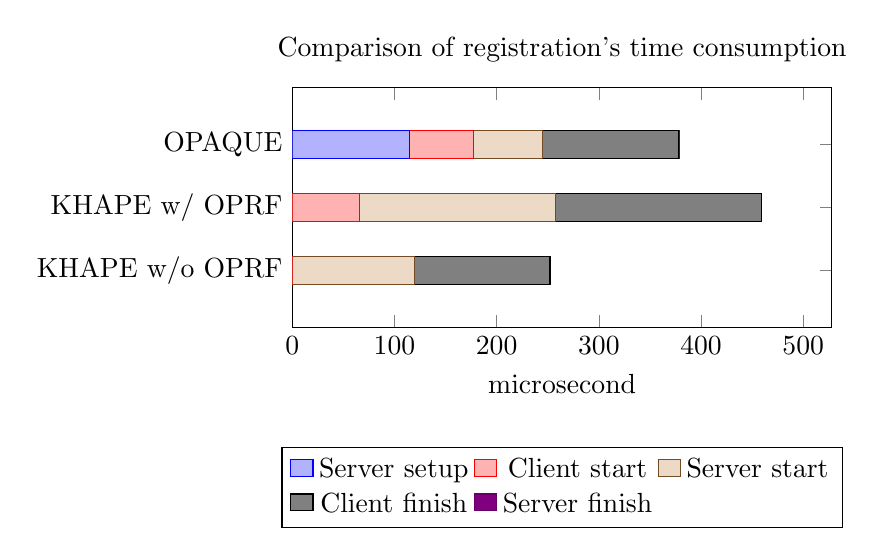
\begin{tikzpicture}
\begin{axis}[
    xbar stacked,
    y=0.8cm,
%     xmin=0, xmax=600,
    enlarge y limits=0.45,
    enlarge x limits={0.15, upper},
    legend style={
        at={(0.5,-0.5)},
        anchor=north
    },
    legend columns=3,
    xlabel={microsecond},
    symbolic y coords={KHAPE w/o OPRF, KHAPE w/ OPRF, OPAQUE},
    ytick=data,
%     nodes near coords,
%     nodes near coords align={vertical},
    title=Comparison of registration's time consumption,
]
\addplot coordinates { % server setup
    (114.80,OPAQUE) (0,KHAPE w/ OPRF) (0,KHAPE w/o OPRF)
};
\addplot coordinates { % client start
    (62.885,OPAQUE) (66.105,KHAPE w/ OPRF) (0.039084,KHAPE w/o OPRF)
};
\addplot coordinates { % server start
    (66.797,OPAQUE) (191.62,KHAPE w/ OPRF) (119.70,KHAPE w/o OPRF)
};
\addplot coordinates { % client finish
    (133.80,OPAQUE) (201.33,KHAPE w/ OPRF) (132.45,KHAPE w/o OPRF)
};
\addplot coordinates { % server finish
    (0.13187,OPAQUE) (0.15336,KHAPE w/ OPRF) (0.15736,KHAPE w/o OPRF)
};
\legend{Server setup, Client start, Server start, Client finish, Server finish}
\end{axis}
\end{tikzpicture}



\subsection*{Authentication}

For the authentication, OPAQUE and KHAPE with OPRF have rather different endpoints performances but the overall performance of each protocol is almost equal with a difference of around 7 us.
This is because a lot of similar operations are computed on both protocol but they are executed in different endpoints.

Similar to the registration, KHAPE without OPRF is the fastest protocol. It is faster by 197 us on OPAQUE and by 205 us on KHAPE with OPRF.
Even if it is the fastest in both registration and authentication, we believe that the security sacrifice is not worth the performance gain and therefore we recommend using OPAQUE or KHAPE with OPRF which are secure against pre-computation attacks (see Section \ref{sec:design_choice_oprf}).


% OPAQUE         : 821.32 us
% KHAPE w/ OPRF  : 830.01 us
% KHAPE w/o OPRF : 624.5 us

% KHAPE w/ - OPAQUE    : 8.69
% OPAQUE - KHAPE w/o   : 196.82
% KHAPE w/ - KHAPE w/o : 205.51
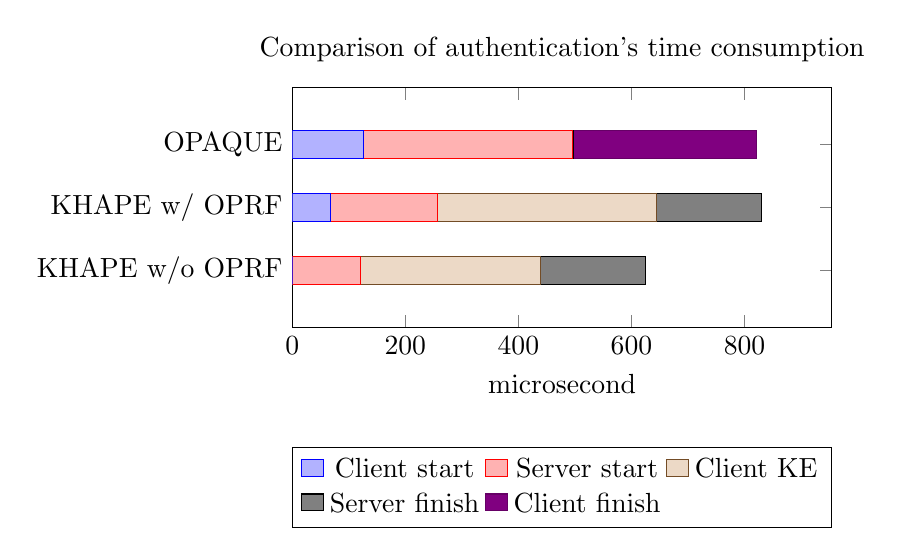
\begin{tikzpicture}
\begin{axis}[
    xbar stacked,
    y=0.8cm,
%     xmin=0, xmax=600,
    enlarge y limits=0.45,
    enlarge x limits={0.15, upper},
    legend style={
        at={(0.5,-0.5)},
        anchor=north
    },
    legend columns=3,
    xlabel={microsecond},
    symbolic y coords={KHAPE w/o OPRF, KHAPE w/ OPRF, OPAQUE},
    ytick=data,
%     nodes near coords,
%     nodes near coords align={vertical},
    title=Comparison of authentication's time consumption,
]
\addplot coordinates { % client start
    (125.40,OPAQUE) (67.308,KHAPE w/ OPRF) (0.039352,KHAPE w/o OPRF)
};
\addplot coordinates { % server start
    (369.59,OPAQUE) (189.93,KHAPE w/ OPRF) (121.29,KHAPE w/o OPRF)
};
\addplot coordinates { % client ke
    (0,OPAQUE) (387.39,KHAPE w/ OPRF) (318.02,KHAPE w/o OPRF)
};
\addplot coordinates { % server finish
    (2.2455,OPAQUE) (185.38,KHAPE w/ OPRF) (185.49,KHAPE w/o OPRF)
};
\addplot coordinates { % client finish
    (324.08,OPAQUE) (0.086069,KHAPE w/ OPRF) (0.085906,KHAPE w/o OPRF)
};
\legend{Client start, Server start, Client KE, Server finish, Client finish}
\end{axis}
\end{tikzpicture}


% KHAPE without OPRF
% \addplot coordinates {
%     (0.085906,client finish)
%     (185.49,server finish)
%     (318.02,client ke)
%     (121.29,server start)
%     (0.039352,client start)
% };


\section{Message size} \label{sec:comp_message_size}

All the above benchmarks are only comparing computational performances by mesuring the time consumption. In a real world scenario, network delay during transmissions of messages between the client and the server also has to be considered. Network delay benchmark is difficult to evaluate and not very meaningful because it depends too much on the network infrastructure between the two parties.

Nevertheless, this section compare the message size and message number for multiple OPAQUE and KHAPE configurations.



OPAQUE results are taken from the standard draft tests vector and verified with the OPAQUE-KE library \cite{OPAQUE-KE}. In these tests vector, the user identifier is 4 bytes long. The same length will be used for KHAPE's uid. It is interesting to note that in OPAQUE, the uid is not transmitted with the protocol's messages. It is the responsibility of the application to handle it. In KHAPE, the uid is included with the protocol's messages and accessible to the application.

For OPAQUE, the message size depends on the primitives used (ciphersuite). In particular, the choice of the hashing function, MAC and KDF has a considerable impact since they can produce output of different length depending on the primitive used.
For the benchmark, we will use a ciphersuite with 256 bit output for hashing function, MAC and KDF because KHAPE also use this output size for these functions. A comparison is also made with a 512 bits output ciphersuite.


Note that the 256 bits ciphersuite use a P256 curve where the points are represented on 33 bytes. The 512 bits ciphersuite use Ristretto255 which is represented on 32 bytes



%                         registration\_request   registration\_response  registration\_upload    KE1         KE2         KE3         KE4
% OPAQUE (512 bits)       64/2=32                 128/2=64                384/2=192               192/2=96    658/2=329   128/2=64
% OPAQUE (256 bits)       66/2=33                 132/2=66                258/2=129               192/2=96    518/2=259   64/2=32
% KHAPE (with OPRF)       4+32=36                 32+32=64                4+64+32=100             4+32=36     64+32+32=128 4+32+32=68 32
% KHAPE (without OPRF)    4+0=4                   32+0=32                 4+64+32=100             4+0=4       64+32+0=96  4+32+32=68  32
% 
% 
% For KHAPE:
% all OPRFs output = 32 bytes
% all group element (priv, pub, field eleme) = 32 bytes



\pgfplotsset{width=\textwidth-2.4cm}


\subsection*{Registration}

Firstly, comparing KHAPE with and without OPRF, we see that the two first message contains 32 more bytes with OPRF. This is simply the size of the representation of a curve point used for OPRF. This difference is exactly the same for the authentication.

Comparing KHAPE and OPAQUE 256 bits ciphersuite, we notice that the last message is larger with OPAQUE.
This is because OPAQUE encrypt the envelope before transmission with a one-time pad key.
This key is derived from a static shared secret which is included in this registration upload message (see Section \ref{sec:opaque_paper_vs_draft}). The difference of size is due to this additional key sent with OPAQUE.


Comparison between the two OPAQUE's ciphersuite, since there is two hashing function derived result
Comparing the two OPAQUE's ciphersuites, we see that the first two messages contains curve point since the 256 bits ciphersuite represent curve points on 33 bytes instead of 32.
The last message contains two hashes derived output. Their size is doubled with the 512 bits ciphersuite.

%%% Registration upload : OK
% OPAQUE:
% - user's public key (group element size)
% - envelope
%   - inner envelope mode (boolean)
%   - nonce (32)
%   - hmac (hash output size)
% - masking key used to mask the envelope (digest output size)
% Total : 

% KHAPE:
% - uid (4)
% - encrypted_envlope (2x 32)
% - pub_a (32)

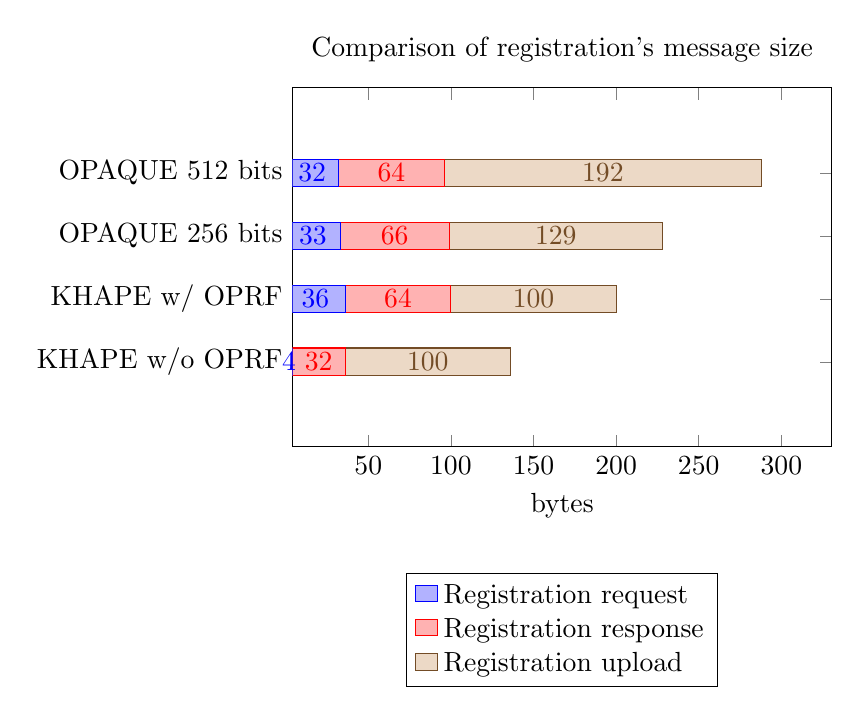
\begin{tikzpicture}
\begin{axis}[
    xbar stacked,
    y=0.8cm,
%     xmin=0, xmax=600,
    enlarge y limits=0.45,
    enlarge x limits={0.15, upper},
    legend style={
        at={(0.5,-0.35)},
        anchor=north
    },
    legend columns=1,
    legend cell align=left,
    xlabel={bytes},
    symbolic y coords={KHAPE w/o OPRF, KHAPE w/ OPRF, OPAQUE 256 bits, OPAQUE 512 bits},
    ytick=data,
    nodes near coords,
%     nodes near coords align={vertical},
    title=Comparison of registration's message size,
]
\addplot coordinates { % registration request
    (32,OPAQUE 512 bits) (33,OPAQUE 256 bits) (36,KHAPE w/ OPRF) (4,KHAPE w/o OPRF)
};
\addplot coordinates { % registration response
    (64,OPAQUE 512 bits) (66,OPAQUE 256 bits) (64,KHAPE w/ OPRF) (32,KHAPE w/o OPRF)
};
\addplot coordinates { % registration upload
    (192,OPAQUE 512 bits) (129,OPAQUE 256 bits) (100,KHAPE w/ OPRF) (100,KHAPE w/o OPRF)
};
\legend{Registration request, Registration response, Registration upload}
\end{axis}
\end{tikzpicture}




\subsection*{Authentication}

For the registration, we can see a relatively large difference between KHAPE and OPAQUE 256 bits ciphersuite in particularly in the second message.
The first message already is about three times longer with OPAQUE. This is because in addition to sending the OPRF blinded element like KHAPE do, OPAQUE also send the client's ephemeral public key and a nonce. KHAPE sends the client's ephemeral public key in the third message.
% TODO client nonce ?
In contrary to the server nonce that is used as a context in key derivation, the client nonce has no use in the OPAQUE's internet standard draft.

For the second message, both OPAQUE and KHAPE sends the encrypted envelope, the OPRF evaluation result and the server's ephemeral public key.
Due to its different envelope encryption (see Section \ref{sec:opaque_paper_vs_draft}), OPAQUE also sends a masking nonce and a the server's public key (which is not included in the envelope in contrary to KHAPE).
OPAQUE also sends a server nonce used in key derivation and the first verification tag.

For the third message, OPAQUE sends the last verification tag where KHAPE only sends the first verification tag with the server ephemeral key.

Only KHAPE sends a fifth message containing the last verification tag.
Even though KHAPE's overall messages size is smaller, the fact that it has one more message 
KHAPE's overall message size is smaller but it has one more message than OPAQUE. Having more message is generally more time consuming than having larger messages with all the overhead of a single message.

Similar to the authentication, KHAPE without OPRF has 32 bytes less for the first two messages than KHAPE with OPRF.


%%% KE1: OK
% OPAQUE: (CredentialRequest)
% - OPRF blinded_element (OPRF group element size)
% - ke1_message
%   - client_nonce (never used, maybe just there to obfusq the ke1 message ?, 32 bytes)
%   - client ephemeral pk (KE group element size)

% KHAPE:
% - uid (4)
% - oprf blind result (32)


%%% KE2: OK
% OPAQUE: (CredentialResponse)
% - OPRF evaluation element (OPRF group element size)
% - masking_nonce (32) "A nonce used for the confidentiality of the masked_response field."
% - masked_response [Npk + Ne] "An encrypted form of the server's public key and the client's Envelope structure."
%   - server public key (KE group element size)
%   - envelope
%     - nonce (32)
%     - auth_tag (hash size)
% - ke2_message
%   - server_nonce (32)
%   - server epehemeral pk (KE group element size)
%   - mac (hash size) "authentication tag computed over the handshake"

% KHAPE:
% - encrypted envelope (2x 32)
% - pub_y (32)
% - oprf evaluation (32)


%%% KE3: OK
% OPAQUE:
% - mac (hash size)

% KHAPE:
% - uid (4)
% - client_verify_tag (32)
% - pub_x (32)


%%% KE4:
% KHAPE:
% - server_verify_tag (32)





%% TODO OPAQUE's envelope
% at register, client compute a masking_key derived from the randomized password like export_key, auth_key and seed but without the nonce
% the client send the masking_key to the server that stores it

% at login, masking_nonce is generated
% record.masking_key is retrieved from storage
% a ephemeral key is computed by HKDF expanding masking_key with masking_nonce
% this ephemeral key is used to xor the [server_public_key and record.envelope] (encryption) the result is called masked_response
% masking_nonce and the masked_response is sent to the client






% what is record.envelope ? envelope contains a nonce and an auth_tag. The auth_tag protect the envelope and the nonce is used to compute auth_key and, export_key and the seed from which the client's private key is derived.

% how client knows masking_key ? masking key is computed by the client at register (like auth_key, export_key and seed but without the nonce) and sent to the server. the server store the masking key


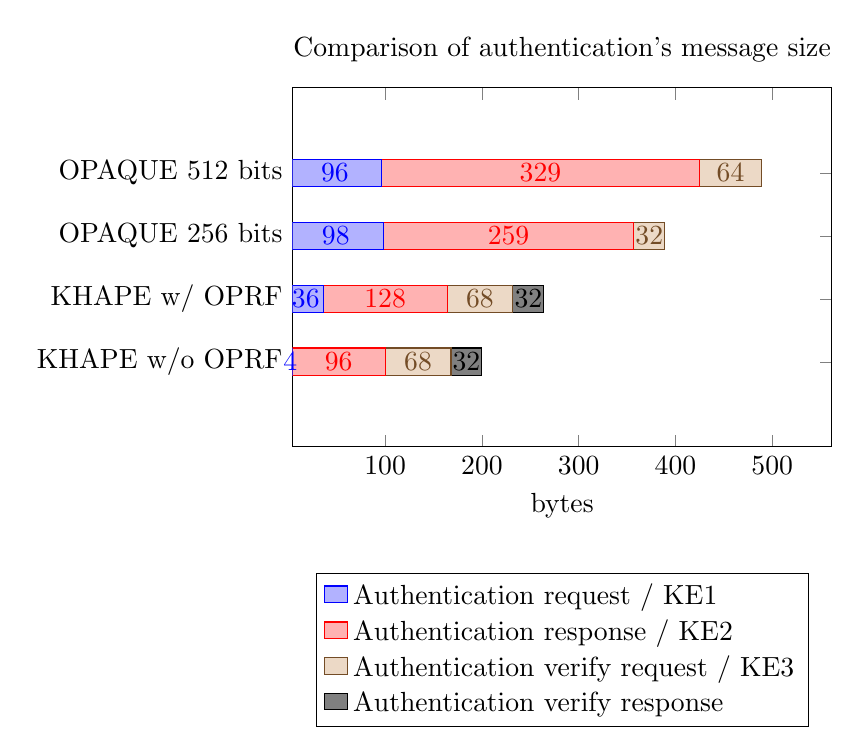
\begin{tikzpicture}
\begin{axis}[
    xbar stacked,
    y=0.8cm,
%     xmin=0, xmax=600,
    enlarge y limits=0.45,
    enlarge x limits={0.15, upper},
    legend style={
        at={(0.5,-0.35)},
        anchor=north
    },
    legend columns=1,
    legend cell align=left,
    xlabel={bytes},
    symbolic y coords={KHAPE w/o OPRF, KHAPE w/ OPRF, OPAQUE 256 bits, OPAQUE 512 bits},
    ytick=data,
    nodes near coords,
%     nodes near coords align={vertical},
    title=Comparison of authentication's message size,
]
\addplot coordinates { % KE1
    (96,OPAQUE 512 bits) (98,OPAQUE 256 bits) (36,KHAPE w/ OPRF) (4,KHAPE w/o OPRF)
};
\addplot coordinates { % KE2
    (329,OPAQUE 512 bits) (259,OPAQUE 256 bits) (128,KHAPE w/ OPRF) (96,KHAPE w/o OPRF)
};
\addplot coordinates { % KE3
    (64,OPAQUE 512 bits) (32,OPAQUE 256 bits) (68,KHAPE w/ OPRF) (68,KHAPE w/o OPRF)
};
\addplot coordinates { % KE4
    (0,OPAQUE 512 bits) (0,OPAQUE 256 bits) (32,KHAPE w/ OPRF) (32,KHAPE w/o OPRF)
};
\legend{Authentication request / KE1, Authentication response / KE2, Authentication verify request / KE3, Authentication verify response}
\end{axis}
\end{tikzpicture}




% \newpage
% 
% 
% \subsection{Registration}
% 
% \pgfplotsset{width=10cm, height=8cm}
% 
% \begin{tikzpicture}
% \begin{axis}[
%     ybar,
%     enlarge x limits=0.15,
%     enlarge y limits={0.15, upper},
%     legend style={at={(0.5,-0.2)},
%     anchor=north,legend columns=-1},
%     ylabel={microseconde},
%     symbolic x coords={client start, server start, client finish, server finish},
%     xtick=data,
%     nodes near coords,
%     nodes near coords align={vertical},
%     x tick label style={rotate=45,anchor=east},
% ]
% \addplot coordinates {
%     (client start,66.105) (server start,191.62) (client finish,201.33)
%     (server finish,0.15336)
% };
% \end{axis}
% \end{tikzpicture}
% 
% 
% \pgfplotsset{width=\textwidth, height=6cm}
% 
% \begin{tikzpicture}
% \begin{axis}[
%     xbar,
%     enlarge y limits=0.2,
%     enlarge x limits={0.15, upper},
%     legend style={at={(0.5,-0.2)},
%     anchor=north,legend columns=-1},
%     xlabel={microseconde},
%     symbolic y coords={server finish, client finish, server start, client start},
%     ytick=data,
%     nodes near coords,
%     nodes near coords align={horizontal},
% ]
% \addplot coordinates {
%     (0.15336,server finish)
%     (201.33,client finish)
%     (191.62,server start)
%     (66.105,client start)
% };
% \end{axis}
% \end{tikzpicture}
% 
% \newpage
% 
% 
% \pgfplotsset{width=\textwidth, height=8cm}
% \usepgfplotslibrary{statistics}
% 
% \subsection{Registration}
% 
% \begin{tikzpicture}
% \begin{axis}[
%     boxplot,
%     boxplot/draw direction=y,
%     xtick={1,2,3,4},
%     xticklabels={client start, server start, client finish, server finish},
%     ylabel={microseconde},
% ]
% \addplot table[y=value]{data/khape_standard/client_register_start.dat};
% \addplot table[y=value]{data/khape_standard/server_register_start.dat};
% \addplot table[y=value]{data/khape_standard/client_register_finish.dat};
% \addplot table[y=value]{data/khape_standard/server_register_finish.dat};
% \end{axis}
% \end{tikzpicture}
% 
% \subsection{Authentication}
% 
% \begin{tikzpicture}
% \begin{axis}[
%     boxplot,
%     boxplot/draw direction=y,
%     xtick={1,2,3,4,5},
%     xticklabels={client start, server start, client ke, server finish, client finish},
%     ylabel={microseconde},
% ]
% \addplot table[y=value]{data/khape_standard/client_auth_start.dat};
% \addplot table[y=value]{data/khape_standard/server_auth_start.dat};
% \addplot table[y=value]{data/khape_standard/client_auth_ke.dat};
% \addplot table[y=value]{data/khape_standard/server_auth_finish.dat};
% \addplot table[y=value]{data/khape_standard/client_auth_finish.dat};
% \end{axis}
% \end{tikzpicture}
% 
% 
% 
% 
% \subsection{Registration}
% 
% \begin{tikzpicture}
% \begin{axis}[
%     boxplot,
%     boxplot/draw direction=x,
%     ytick={1,2,3,4},
%     yticklabels={client start, server start, client finish, server finish},
%     xlabel={microseconde},
% ]
% \addplot table[y=value]{data/khape_standard/client_register_start.dat};
% \addplot table[y=value]{data/khape_standard/server_register_start.dat};
% \addplot table[y=value]{data/khape_standard/client_register_finish.dat};
% \addplot table[y=value]{data/khape_standard/server_register_finish.dat};
% \end{axis}
% \end{tikzpicture}
% 
% \subsection{Authentication}
% 
% \begin{tikzpicture}
% \begin{axis}[
%     boxplot,
%     boxplot/draw direction=x,
%     ytick={1,2,3,4,5},
%     yticklabels={client start, server start, client ke, server finish, client finish},
%     xlabel={microseconde},
% ]
% \addplot table[y=value]{data/khape_standard/client_auth_finish.dat};
% \addplot table[y=value]{data/khape_standard/server_auth_finish.dat};
% \addplot table[y=value]{data/khape_standard/client_auth_ke.dat};
% \addplot table[y=value]{data/khape_standard/server_auth_start.dat};
% \addplot table[y=value]{data/khape_standard/client_auth_start.dat};
% \end{axis}
% \end{tikzpicture}
% 
% 
% \newpage
% 
% 
% \pgfplotsset{width=4cm, height=8cm}
% \begin{tikzpicture}
% \begin{axis}[
%     boxplot,
%     boxplot/draw direction=y,
%     ylabel={us},
% ]
% \addplot table[y=value]{data/khape_standard/client_auth_start.dat};
% \end{axis}
% \end{tikzpicture}
% 
% 
% \begin{tikzpicture}
% \begin{axis}[
%     boxplot,
%     boxplot/draw direction=y,
%     ylabel={us},
% ]
% \addplot table[y=value]{data/khape_standard/server_auth_start.dat};
% \end{axis}
% \end{tikzpicture}
% 
% 
% \pgfplotsset{width=10cm, height=4cm}
% \begin{tikzpicture}
% \begin{axis}[
%     boxplot,
%     boxplot/draw direction=x,
%     xlabel={us},
% ]
% \addplot table[y=value]{data/khape_standard/client_auth_start.dat};
% \end{axis}
% \end{tikzpicture}
% 
% 
% \begin{tikzpicture}
% \begin{axis}[
%     boxplot,
%     boxplot/draw direction=x,
%     xlabel={us},
% ]
% \addplot table[y=value]{data/khape_standard/server_auth_start.dat};
% \end{axis}
% \end{tikzpicture}

\end{document}

